\documentclass[twocolumn]{revtex4}
\usepackage{graphics,graphicx,epsfig,ulem,amsmath,multirow,gensymb,commath,textcomp,natbib}
\newcommand{\squeezeup}{\vspace{-2.5mm}}

\begin{document}

\textheight=26.385cm
%Change textheight as the last resort...

\title{Investigating and understanding Fraunhofer diffraction patterns using Fourier analysis with variations of the 4f Optical System}
 
\author{Jacky Cao, Room 205, Friday, Lab Partners: Thomas Spriggs \\ Date of experiment: 10/02/2017 to 17/03/2017, Date of report: 19/03/2017}

\begin{abstract}              
Through the study of the Fourier Transforms of blah blah blah. \cite{crc}. 
\end{abstract}

\maketitle

\section{Introduction} 
\vspace{-2ex} 

In the field of optics, a Fraunhofer diffraction pattern can be produced when a coherent beam of radiation falls onto a partially opaque object \cite{mathmethods}. The pattern can then be viewed at a ``far-field'' distance, this length being larger than the initial size of the object, allowing for the spreading of light due to diffraction to dominate in the observation plane \cite{of2f}. 

The usage of diffraction patterns includes the studying of crystalline structures. Through X-ray and electron diffraction it is possible to obtain accurate information about the identity of phases present, atomic ordering, and for recognising different metallurgical constituents within a specimen. This allows for potential applications within the pharmaceutical industry for example, where early analysis of different mixtures and compounds can be cost and time saving. \cite{elecdiffraction, xraypharma}

Another application could potentially involve using the diffraction pattern within an illumination system so that x-ray phase contrast microscopy and interferometry can be performed \cite{singleslit}. This could be used to enhance the visibility of fine scale structures, this being especially useful in biology as quantitative information can be obtained about a sample from just phase-contrast images \cite{xrayphase}.

With these varying applications we find that in order to fully understand diffraction patterns and how they form, we must look at the mathematics behind them. 

The main mathematical tool that we must use in building our understanding is Fourier analysis, more specifically, Fourier transforms. A Fourier transform is a way to represent a function in terms of a superposition of sinusoidal functions, with the explicit conditions of the function being defined over an infinite interval and having no particular periodicity \cite{mathmethods}.

The Fourier transform $F(u)$ of a single function $f(x)$ can be stated as,
\begin{equation}
F(u) = \mathcal{F}[f(x)](u) = \int_{-\infty}^\infty f(x) e^{-i2\pi ux}dx,
\end{equation}

where $(u)$ is the dependent Fourier variable. This expression tells us the spectrum of frequencies required to form the function $f(x)$ \cite{of2f}.

In optics, the Fourier variable used above is called the spatial frequency, $u$. It is defined as the \textsl{number of waves per unit length} - the real space analogue of frequency. It's mathematical form for the far-field case can be written as a mapping between the Fourier variable and real space position,
\begin{equation}
u=\frac{x}{\lambda z},
\end{equation}

where $x$ is the position in real space, $\lambda$ is the wavelength of radiation being used to illuminate the object, and $z$ is the distance 'downstream' from the object \cite{of2f}.

There are also extensions of this for 

his is especially the case when the cross-section of the object is small when compared with the  For example a laser shining upon a diffraction grating can produce


\vspace{-3ex}
\section{Method} 
\vspace{-2ex}

Method

\begin{figure}[!h]
\begin{center}
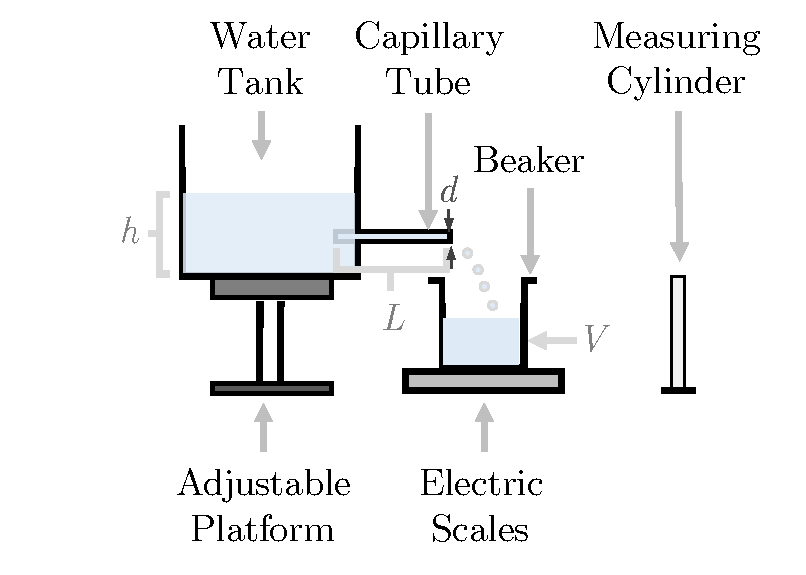
\includegraphics[width=5.7cm]{results/fig1}
\caption[]{A schematic of the experimental set-up used to collect data. }
\label{fig:fig1}
\end{center}
\end{figure}

Method

\vspace{-3ex}
\section{Results}
\vspace{-2ex}

Results

\begin{table}[h!]
\centering
\begin{tabular}{c@{\hskip 20pt}c@{\hskip 20pt}c@{\hskip 20pt}c} 
 \hline
 \textbf{Tube} & \textbf{Radius, a [mm]} & \textbf{$\boldsymbol{\eta}$ [mPa {s}]} & \textbf{$\boldsymbol{\chi^2_{\nu}}$} \\ [0.5ex] 
 $Blue$ &$0.55\pm0.03$ & $1.0\pm0.2$ & 11.0 \\ 
 $Red$ & $0.47\pm0.03$ & $1.1\pm0.3$ & 5.31 \\
 $Black$ & $0.46\pm0.03$ & $1.0\pm0.3$ & 1.94 \\
 
 \hline
\end{tabular}
\caption{For each tube is shown its radius, their respective calculated value for the viscosity of water $\eta$, and the reduced chi-squared statistic, $\chi^2_{\nu}$.}
\label{table:1}
\end{table}

\vspace{-3ex}
\section{Discussion}
\vspace{-2ex}

Discussion

\vspace{-5ex}
\section{Conclusions}
\vspace{-2ex}

Conclusion

\begin{thebibliography}{5}
\bibitem{mathmethods}
	K. F. Riley, M. P. Hobson, and S. J. Bence.
	\textit{Mathematical Methods for Physics and Engineering}.
	Cambridge University Press, Cambridge, UK, 2010.
	
\bibitem{of2f}
	C. S. Adams and I. G. Hughes.
	\textit{Optics f2f, from Fourier to Fresnel}.
	Clarendon Press, Oxford, UK, 2017.

\bibitem{elecdiffraction}
	K. W. Andrews, D. J. Dyson, and S. R. Keown.
	\textit{Interpretation of Electron Diffraction Patterns}.
	Hilger \& Watts Ltd, London, UK, 1967.
	
\bibitem{xraypharma}
	J. P. Smit, R. B. McClurg.	
	\textit{X-ray Powder Diffraction Pattern Indexing for Pharmaceutical Applications}.
	Pharmaceutical Technology, January 2013, Vol. 37, No. 1.
	
\bibitem{singleslit}
	A. R. Lang, et al.
	\textit{Single-slit diffraction patterns of sub-nanometre-wavelength synchrotron radiation}.
	Journal of Physics D: Applied Physics, 1987, Vol. 20, No. 4, pp. 541-544.
	
\bibitem{xrayphase}
	S. C. Mayo, et al.
	\textit{X-ray phase-contrast microscopy and microtomography}.
	Optical Express, 2003, Vol. 11, No. 19, pp. 2289-2302.

\bibitem{youngandfreedman} 
	Hugh D. Young and Roger A. Freedman.
	\textit{University Physics with Modern Physics, 13th Edition}. 
	Pearson Education Limited, Essex, UK, 2015.
	
	
\bibitem{hughesandhayes} 
	I. G. Hughes and T. P. A. Hase.
	\textit{Measurements and their Uncertainties}. 
	Oxford University Press, Oxford, UK, 2010.
	
\end{thebibliography}
\clearpage

\vfill
\twocolumngrid
\vspace{-3ex}
\section*{Appendix}
\vspace{-2ex}

Appendix


\clearpage
\end{document}